\documentclass[conference,12pt]{IEEEtran}
%DIF LATEXDIFF DIFFERENCE FILE
%DIF DEL ..\..\proposal\proposal.tex   Sat Mar  8 21:17:55 2014
%DIF ADD proposal.tex                  Sun Mar  9 22:19:36 2014
\usepackage{pdflscape}
\usepackage{hyperref}
\usepackage{tabularx}
\usepackage{graphicx, subfigure, amsmath} 
%DIF 6a6
\usepackage{pdfpages} %DIF > 
%DIF -------
\usepackage[backend=biber,style=ieee]{biblatex}
\usepackage[section]{placeins}
\addbibresource{References/References.bib}
\interdisplaylinepenalty=2500

% correct bad hyphenation here
\hyphenation{}
%DIF PREAMBLE EXTENSION ADDED BY LATEXDIFF
%DIF UNDERLINE PREAMBLE %DIF PREAMBLE
\RequirePackage[normalem]{ulem} %DIF PREAMBLE
\RequirePackage{color}\definecolor{RED}{rgb}{1,0,0}\definecolor{BLUE}{rgb}{0,0,1} %DIF PREAMBLE
\providecommand{\DIFaddtex}[1]{{\protect\color{blue}\uwave{#1}}} %DIF PREAMBLE
\providecommand{\DIFdeltex}[1]{{\protect\color{red}\sout{#1}}}                      %DIF PREAMBLE
%DIF SAFE PREAMBLE %DIF PREAMBLE
\providecommand{\DIFaddbegin}{} %DIF PREAMBLE
\providecommand{\DIFaddend}{} %DIF PREAMBLE
\providecommand{\DIFdelbegin}{} %DIF PREAMBLE
\providecommand{\DIFdelend}{} %DIF PREAMBLE
%DIF FLOATSAFE PREAMBLE %DIF PREAMBLE
\providecommand{\DIFaddFL}[1]{\DIFadd{#1}} %DIF PREAMBLE
\providecommand{\DIFdelFL}[1]{\DIFdel{#1}} %DIF PREAMBLE
\providecommand{\DIFaddbeginFL}{} %DIF PREAMBLE
\providecommand{\DIFaddendFL}{} %DIF PREAMBLE
\providecommand{\DIFdelbeginFL}{} %DIF PREAMBLE
\providecommand{\DIFdelendFL}{} %DIF PREAMBLE
%DIF END PREAMBLE EXTENSION ADDED BY LATEXDIFF
%DIF PREAMBLE EXTENSION ADDED BY LATEXDIFF
%DIF HYPERREF PREAMBLE %DIF PREAMBLE
\providecommand{\DIFadd}[1]{\texorpdfstring{\DIFaddtex{#1}}{#1}} %DIF PREAMBLE
\providecommand{\DIFdel}[1]{\texorpdfstring{\DIFdeltex{#1}}{}} %DIF PREAMBLE
%DIF END PREAMBLE EXTENSION ADDED BY LATEXDIFF

\begin{document}
%
% paper title
\title{RoboTractor: A Secure Signaling and Control System for Remote Management of Agricultural Vehicles using XMPP and REST}

\author{
\IEEEauthorblockN{Jeremy Wright}
\IEEEauthorblockA{Arizona State University\\jlwrigh1@asu.edu}
\and
\IEEEauthorblockN{Arun Balaji Buduru}
\IEEEauthorblockA{Arizona State University\\abuduru@asu.edu}
\and
\IEEEauthorblockN{David Lucero}
\IEEEauthorblockA{Arizona State University\\dwlucero@asu.edu}
}
\maketitle


\begin{abstract}
The need for the automation of vehicles is increasing \DIFdelbegin \DIFdel{due to
improved efficiency}\DIFdelend \DIFaddbegin \DIFadd{requiring
improved efficiency, operation, }\DIFaddend and reduced operational costs. The scope of this
project is to build a \DIFdelbegin \DIFdel{secure }\DIFdelend signaling and control system with
\DIFdelbegin \DIFdel{mechanisms }\DIFdelend \DIFaddbegin \DIFadd{a focus on security, in order }\DIFaddend to drastically reduce \DIFdelbegin \DIFdel{if not eliminate the secure signal
and control }\DIFdelend \DIFaddbegin \DIFadd{the }\DIFaddend systems from being \DIFdelbegin \DIFdel{are compromised, making automated
vehicles vulnerable }\DIFdelend \DIFaddbegin \DIFadd{compromised.
An attack against these systems could allow for the vehicles }\DIFaddend to be stolen, damaged, \DIFdelbegin \DIFdel{or otherwise harm the
environment}\DIFdelend \DIFaddbegin \DIFadd{hijacked, or cause other losses}\DIFaddend .
The main tasks in this project are to build a \DIFaddbegin \DIFadd{secure }\DIFaddend front-end
\DIFaddbegin \DIFadd{web }\DIFaddend interface for users to give instructions\DIFaddbegin \DIFadd{, }\DIFaddend built upon a Representational
State Transfer (REST) architecture, set up \DIFaddbegin \DIFadd{an }\DIFaddend Extensible Messaging and
Presence Protocol (XMPP) server and client with required
authentication\DIFdelbegin \DIFdel{and }\DIFdelend \DIFaddbegin \DIFadd{, }\DIFaddend data integrity check mechanisms \DIFaddbegin \DIFadd{and encryption}\DIFaddend , and build a
simulated automated vehicle, capable of interfacing with the XMPP
components and front-end.
\end{abstract}

\begin{IEEEkeywords}
    Secure signaling and control, remote management, agricultural vehicles
    automation, self-driven vehicles\DIFaddbegin \DIFadd{, TPM, root of trust, trusted platform,
    TrustZone, ARM, machine automation
}\DIFaddend \end{IEEEkeywords}

\section{Introduction}
\DIFaddbegin \IEEEPARstart{A}{griculture} \DIFadd{has a growing problem. Crop input costs such as water,
fertilizer, pesticides, and fuel, are increasing. The global population is
increasing driving the need for more food. Local, State, and Federal governments
are increasing oversight and reporting requirements on growers. Land area
available for planting, and harvesting is decreasing globally. All this pushes
farmers to rely on technology to improve their efficiency while reducing
recurrent costs. Take government oversight requirements
}\autocite{_growers_oversight}\DIFadd{, growers are required to track where, and how much
material is spread into the fields.  This can be a considerable overhead for
growers, however an automated machine can do this quite easily, and in real-time
if  desired.  This project demonstrates how to securely connect an agricultural
machine to an automation server in a secure manner using existing internet
technologies. Using existing technologies is a critical point. The market is
already stretched thin, and incurring new infrastructure in rural areas can be
prohibitively expensive, however leveraging the existing Internet infrastructure we
can provide high levels of service in a secure manner.
}

\DIFaddend The most important requirement in developing a secure signal and control
system is ensuring authentication of vehicles and data integrity, \DIFdelbegin \DIFdel{here
the }\DIFdelend \DIFaddbegin \DIFadd{and securing communication channels.
The }\DIFaddend path plan and location feedback transmission needs to be secured
and protected from eavesdroppers, preventing attackers from
compromising and/or stealing these vehicles. In this project we use
\DIFdelbegin \DIFdel{Django }\DIFdelend \DIFaddbegin \DIFadd{the Django web framework }\DIFaddend to handle the front end interface \DIFdelbegin \DIFdel{for the users. 
We use python
libraries }\DIFdelend \DIFaddbegin \DIFadd{and server duties. 
Django facilitates the use of python libraries and components }\DIFaddend to interface between \DIFdelbegin \DIFdel{user and path generator serverwhere we
use XMPP and REST protocols, and XMPP clients to control the
agricultural vehicles.
We expect }\DIFdelend \DIFaddbegin \DIFadd{our Front-end, server, and client-side vehicle simulators.
The end-goal of RoboTractor is }\DIFaddend to have a comprehensive tool that
translates the abstract user inputs into \DIFaddbegin \DIFadd{remotely }\DIFaddend executable actions for
agricultural vehicles in a secure manner \DIFdelbegin \DIFdel{.
}\DIFdelend \DIFaddbegin \DIFadd{using advanced web, network, and cryptographic techniques.
}

\DIFadd{RoboTractor is a framework to provide integrity, authentication, and root of
trust services for machine automation specifically within an agriculture domain.
Electronic Control Unit (ECU) manufacturers will particularly be interested in the root-of-trust details
described in Section~\ref{sec:xmpp}.  Agricultural service providers have
typically be subject to locality issues. Historically, it's been difficult to
provide agricultural services at a reasonable cost, at any appreciable distance
from the farm itself.  RoboTractor provides a conduit for service providers to
provide their services at a distance. This allows expert agronomists to consult
with farms at any distance.  Not only can this reduce cost, but it also allows
growers access to a marketplace of services before unavailable to them.
RoboTractor is the foundation for connecting the needs of the growers to the
providers.  
}

\DIFaddend \section{System Models}

\subsection{System Model}
RoboTractor will leverage the Django Web framework \autocite{_django_2014}
, to realize the required
interfaces.  Figure~\ref{fig:softwarecomponents} describes the connection of
these components.  The combination of XMPP and REST in RoboTractor is
a demonstration of how to extend the existing HTTP development environment
i.e. "the web of things" into a stateful protocol. HTTP is by design
stateless. XMPP on the other hand is a stateful streaming connection between two
clients. In this case the Tractor and a command server.  To achieve this mesh we
will leverage the Bidirectional-streams Over Synchronous HTTP standard
protocol \autocite{paterson_bidirectional-streams_2010}. BOSH provides
a standard mechanism to operate the streaming XMPP protocol efficiently over an
HTTP connection. This is essential for a scalable webservice. 
\subsection{Software}
\subsubsection{XMPP Server}
RoboTractor uses the ejabberd \autocite{_ejabberd} XMPP server as it provides an existing Python
interface, to integrate with the rest of our Python based ecosystem.
\subsubsection{REST Interface}
TastyPie provides REST \autocite{_toastdriven/django-tastypie_2014} by extending
the existing Django Models.
\subsubsection{BOSH Interchange}
Punjab is an Django plugin implementation of BOSH
\autocite{_twonds/punjab_2014}.  In addition to BOSH, this library combines
the ejabberd Users with Django Users to provide a single authentication and
authorization framework. While this demo project will have a single user type,
this combination is critical to maintain proper use management and
least-privilege authorization.

\begin{figure}
\centering
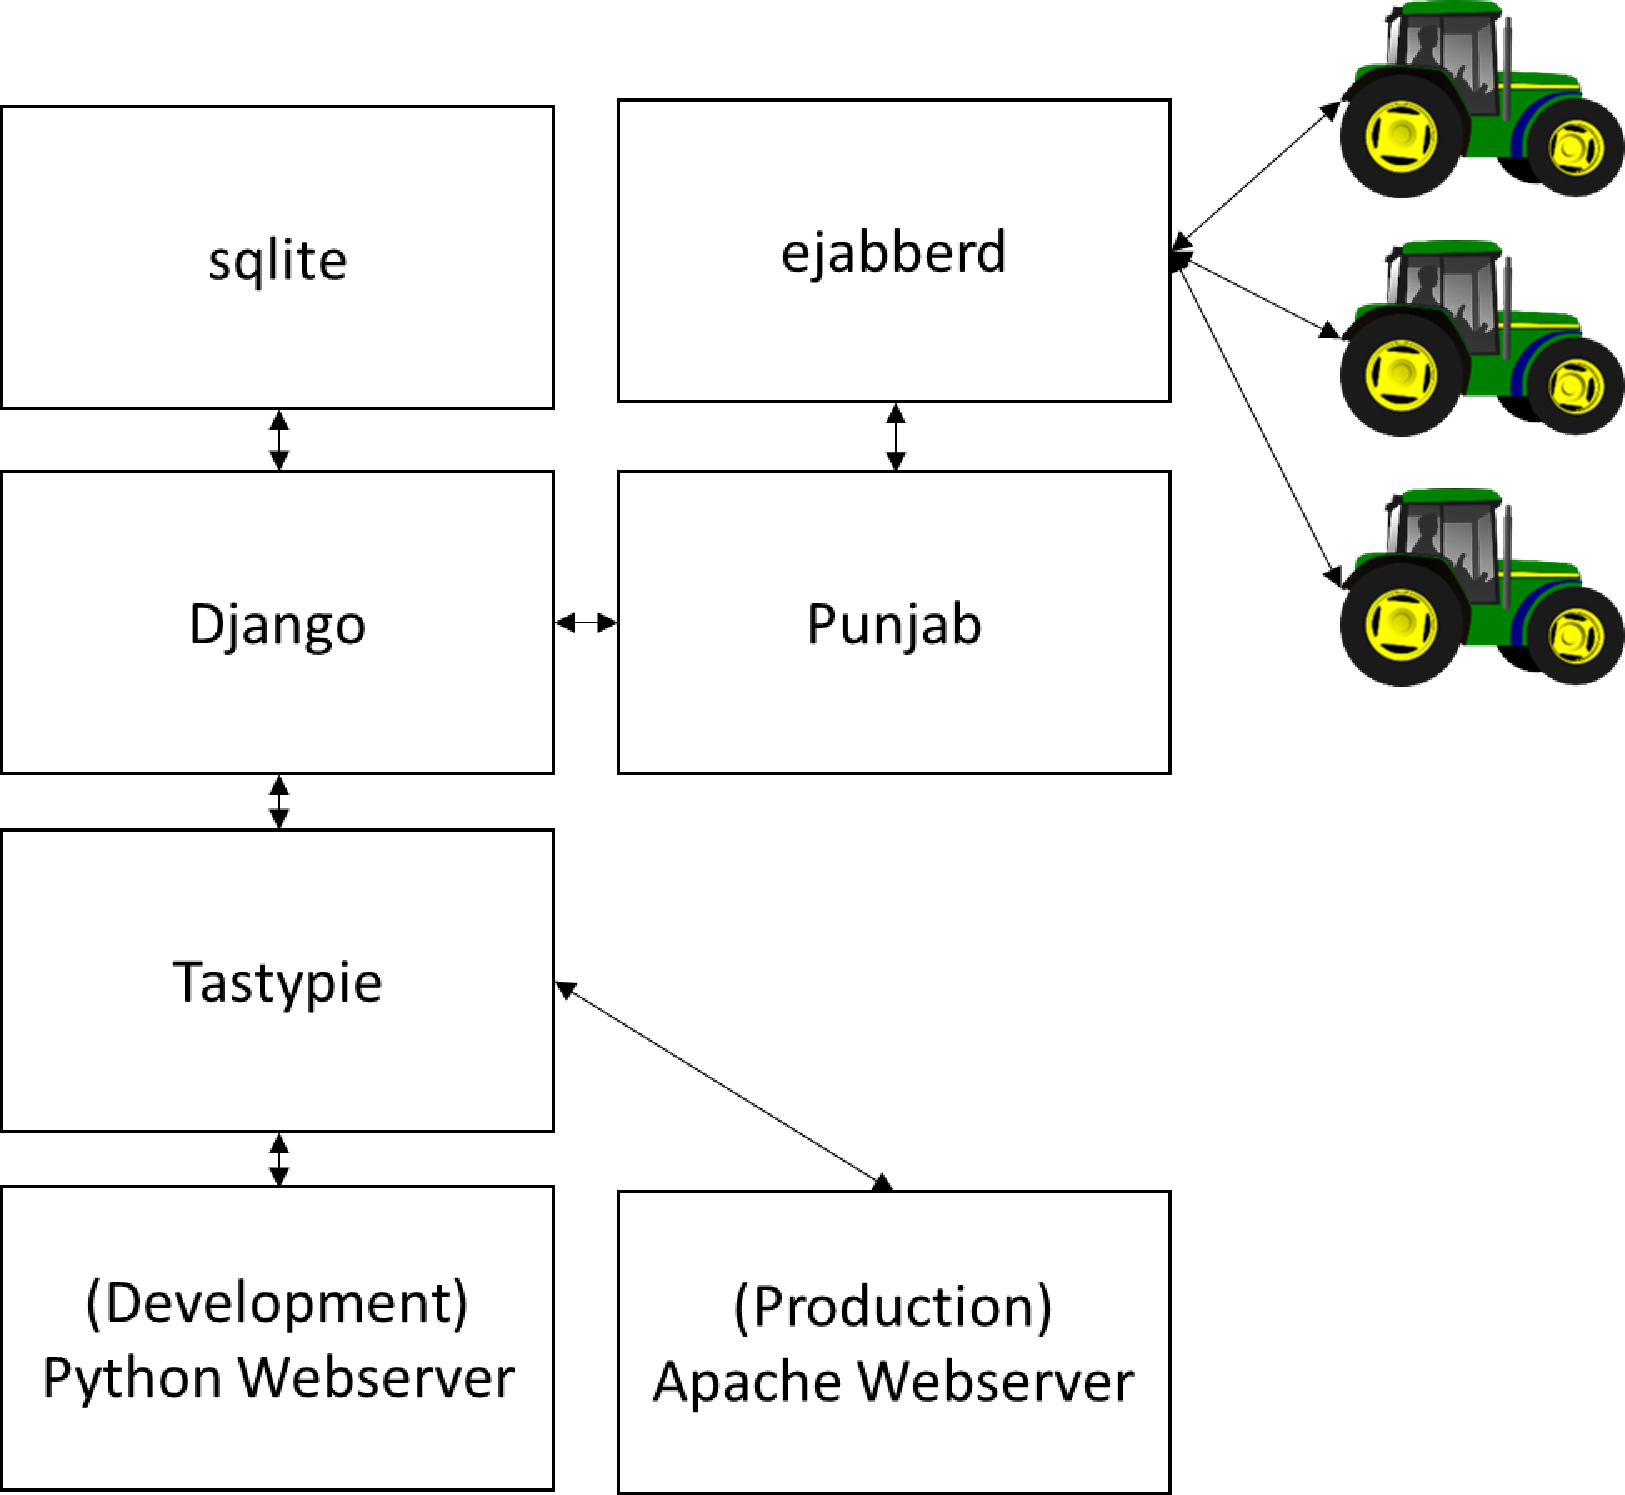
\includegraphics[width=0.4\textwidth]{SoftwareComponentBlockDiagram.pdf}
\caption{Software Component Block Diagram}
\label{fig:softwarecomponents}
\end{figure}

\subsection{Security Model}
RoboTractor deals with two primary security classes: One involving the vehicles
and other assets, and one involving the system components and their communication channels.
Because the project is web-based and uses PKI, numerous attack models have
been created that this project will deal with. Within the class of communication channels,
attacks may be present against the authentication systems of both users and assets. Robotractor \DIFdelbegin \DIFdel{will employ
}\DIFdelend \DIFaddbegin \DIFadd{currently employs
}\DIFaddend advanced two-factor authentication. Usage of TLS and other best common practices will \DIFdelbegin \DIFdel{help }\DIFdelend \DIFaddbegin \DIFadd{be implemented }\DIFaddend to prevent
against replay attacks on the system, and also for establishing a secure session between assets and control.
A dual-encryption scheme has been devised to send encrypted control signals within an encrypted XMPP stanza
to ensure high information assurance. Because this project will utilize PKI, key protection is important. To this end
the RoboTractor project plans to secure keys on assets with a Trusted Platform Module or relevant simulated facsimile.
By making both key-pairs private and secure, RoboTractor provides advanced communication security.
On the other end, the server components must be secured as well using best common practices in server defense, firewall,
patches, updates, etc. Additionally, the RoboTractor system will implement an advanced GPS location reporting system
to provide physical security in case of asset theft. By defending against these attack models, the RoboTractor project
presents the realization of an advanced system for signaling and control with high security. 

\section{Project Description}
\DIFaddbegin \label{sec:proj_desc}
\DIFaddend Implementation is divided into 2 primary phases (Marked as milestones on the
attached Gantt chart).  The first phase is an integration phase connecting
the various libraries and off the shelf components. It is critical that this
integration does not weaken, but rather strengthens the security properties
provided by each independent component. 

\DIFaddbegin \begin{figure}
\centering
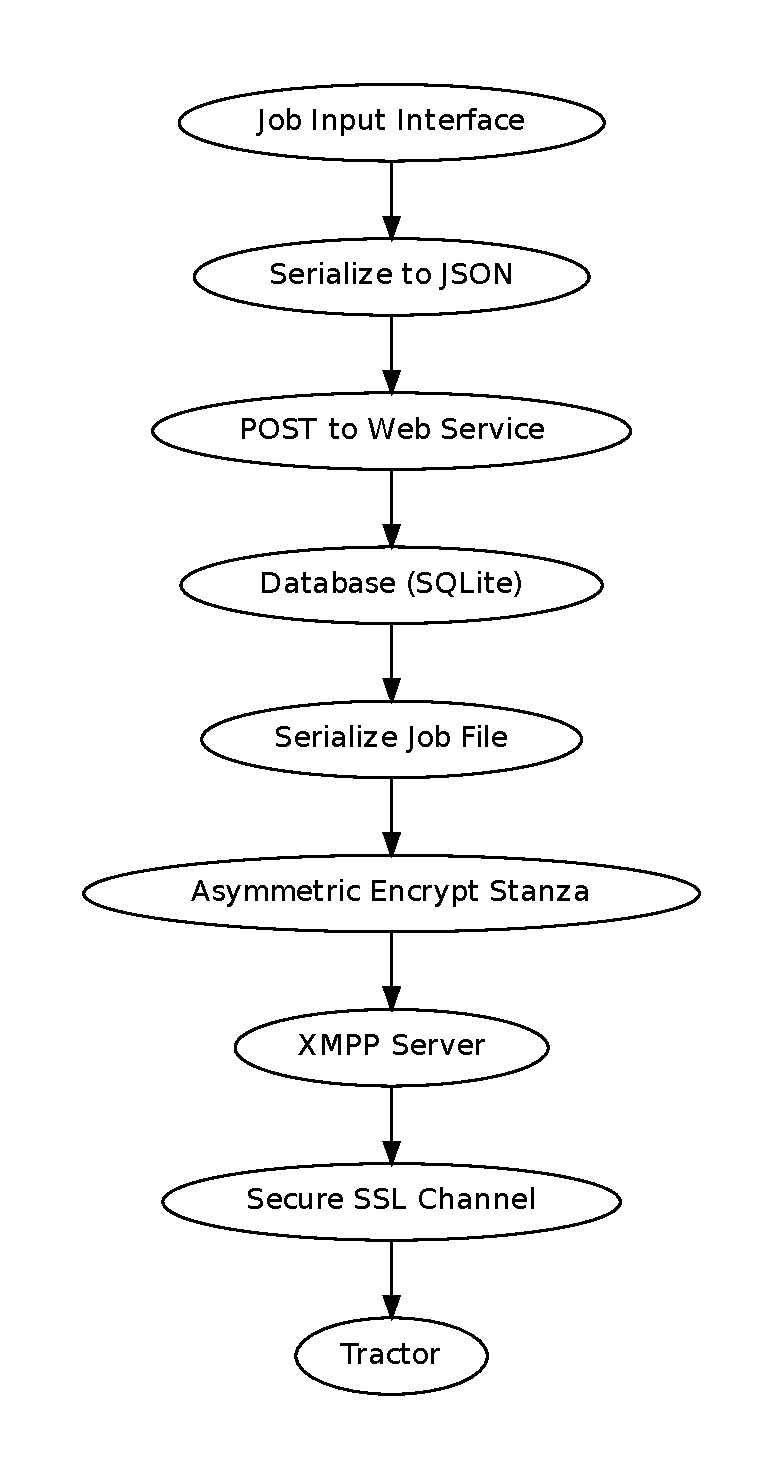
\includegraphics[width=0.4\textwidth]{signalpath.pdf}
\caption{\DIFaddFL{High Level Signal Path}}
\label{fig:signalpath}
\end{figure}


\DIFaddend The second phase is the extension of these components to provide command and
control of agricultural vehicles. For schedule mitigation, David and Arun are
scheduled to begin this phase before the framework is assembled. Once the
framework is in place, David and Arun's interface designs may be merged with the
overall system. \DIFdelbegin \subsection{\DIFdel{Task 1 : Development Environment}}
%DIFAUXCMD
\addtocounter{subsection}{-1}%DIFAUXCMD
\DIFdel{The development environment consists of configuring all the tools needed to portably work with the software package. This will involve installing project dependencies, and deployment scripts to allow all members of
the team to work
effectively together. 
The complete environment will be stored in git. }\DIFdelend \DIFaddbegin \DIFadd{As of the creation of this document, all Midterm deliverables have been achieved.
The following tasks have been updated to reflect work currently done, and remaining future work.
}

\subsection{\DIFadd{Task 1 : Development Environment}}
\DIFadd{This task consisted of setting up the development environment for the RoboTractor project. 
A project homepage was provided to us via the ASU virtual lab project. This home page provides
source control in the form of a GIT repository which our project takes advantage of. Additionally, two
virtual machines were provided via the ASU virtual lab project to use as our project servers. Setup of
these servers was automated with the creation of a script in order to download all required software packages.
Remaining work for this task is to enable proper connectivity between the two
assigned Virtual Machines. 
}

\DIFadd{RoboTractor on built on the Django. The development environment is best
described in }\autocite{_django_2014}\DIFadd{. The Development environment consists of
2 Fabric configurations one for development and a second for deployment. This
  allows development settings to be more relaxed facilitating quick coding
  cycles, while the deployed configuration is more secure. Separate database
  also prevent test data from polluting the deployed demo project.
}

\DIFaddend \subsection{Task 2: XMPP Implementation}
\DIFaddbegin \label{sec:xmpp}
\DIFaddend XMPP Implementation is a configuration task to setup the ejabberd server and
connect it into the HTTP Framework. \DIFdelbegin \DIFdel{Once this is in place the XMPP
Clients may start working.  }\DIFdelend \DIFaddbegin \DIFadd{The XMPP client/server components and
interfacing with them is not a midterm deliverable, and is to be finished before
final submission.
}

\DIFadd{XMPP provides an SSL/TLS connection between the tractor, and the server. This
allows a base level of secure communication.  However to augment the security
model, we provide additional asymmetric encryption of the command structures
in each XMPP stanza.  This also leverages a Trusted Platform
Module (TMP). TMP is a hardware module, either part of the compute engine
complex or as in ARM processors integrated into the CPU core itself.  ARM's
offering is called TrustZone.  These security services provide a hardened
storage location for private keys.  One cannot extract the key without
destroying the device, and the key itself.  These devices also leverage a best
practice called ``Root of Trust'' to protect against known cipher attacks
}\autocite{_tpm_2013}\DIFadd{.  The
hardware modules only decrypt/encrypt material if the system is in a ``secure''
state.  Typically this is obtained by the compute core booting an internal,
untamperable ROM loader.  This loaders verifies the second stage bootloader with
a cryptographic signature stored in the TPM device at production time. If this
signature passes, the TPM is unlocked and the hardware may continue booting. If
any signature fails, the TPM remains locked, and refused to cipher information.
For the purposes of RoboTractor this behavior will be simulated at the API
level.  However hardware integrators may leverage the best practices laid out
here to implement a ``root of trust'' to include the automation server.  
}

\DIFaddend \subsection{Task 3: Demo Tractor}
\DIFdelbegin \DIFdel{The Demo tractor is the complementary component to the Frontend UI.  This is the
virtual machine,
a piece of software which simulates a real tractor , or
agricultural vehicle }\DIFdelend \DIFaddbegin 

\begin{figure}
\centering
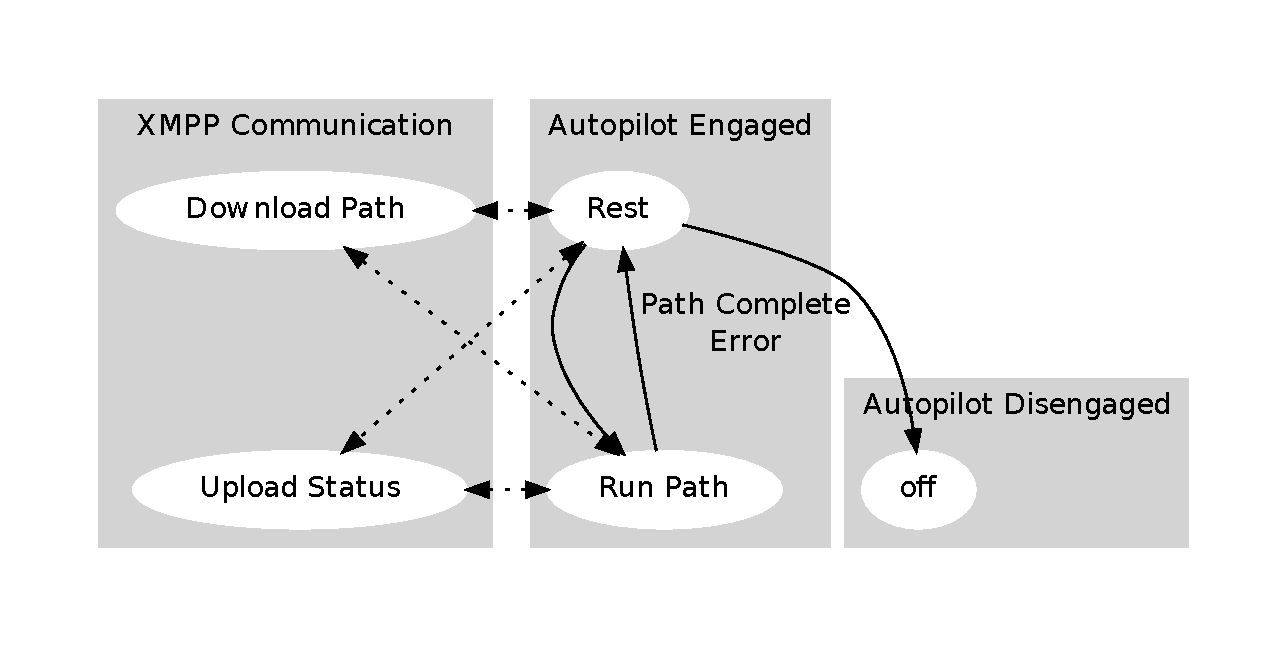
\includegraphics[width=0.4\textwidth]{machine.pdf}
\caption{\DIFaddFL{Tractor Software State Machine}}
\label{fig:tractorstatemachine}
\end{figure}
\DIFadd{The midterm deliverable for this task was to finalize the design specifications
of the tractor simulator. This has been achieved after multiple team
discussions, and a basic state machine vehicle simulator has been written in
python. As more tasks are completed, the simulator is to be updated with its
required functionality such as XMPP communication, path processing, and status
reporting. The state machine consumes the Job File format described in
Figure~\ref{fig:jobfile}.  
}

\begin{figure}
\centering
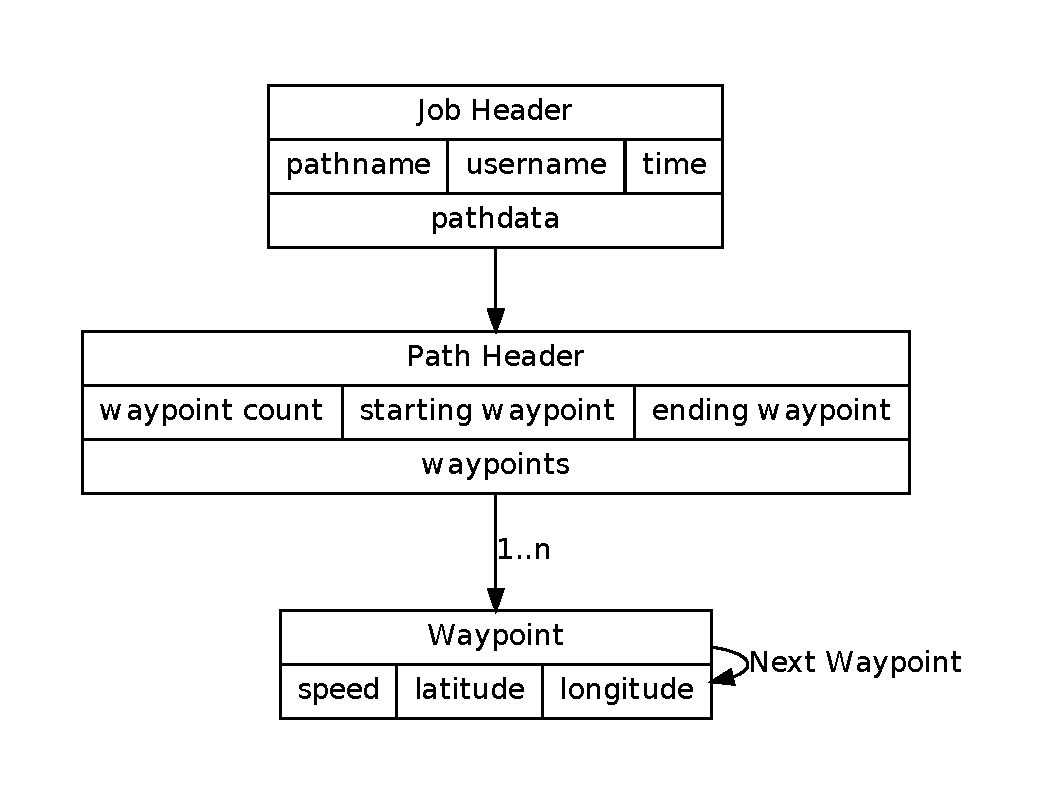
\includegraphics[width=0.4\textwidth]{job_file.pdf}
\caption{\DIFaddFL{Job File Format}}
\label{fig:jobfile}
\end{figure}

\DIFadd{As described in Figure~\ref{fig:signalpath}, the job files are stored in the
database. When the Tractor is instructed to run a job, the Tractor downloads the
Job file from the server over its XMPP connection. The backend server is
responsible for translating the database models into JSON encoded Job
File }\autocite{_json_2014}\DIFaddend .
\DIFaddbegin 

\DIFaddend \subsection{Task 4: Frontend UI}
\DIFaddbegin \begin{figure}
\centering
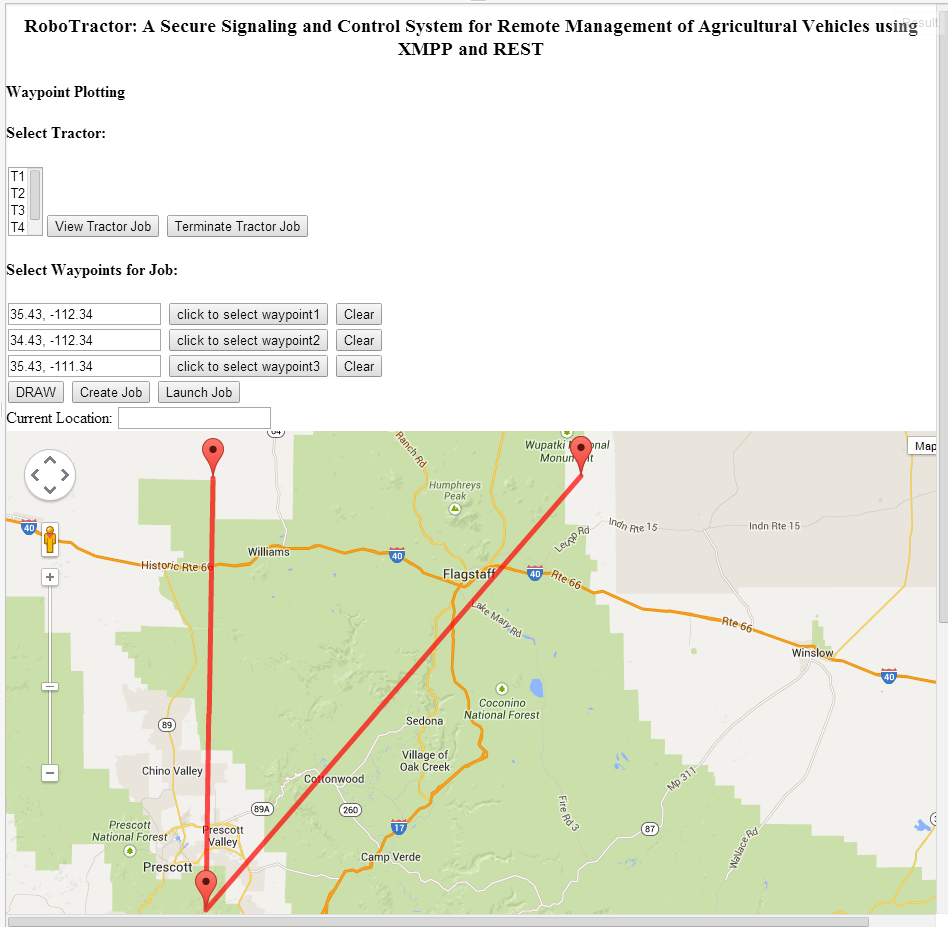
\includegraphics[width=0.4\textwidth]{../PlottingV1.png}
\caption{\DIFaddFL{Job Input Tool}}
\label{fig:jobinput}
\end{figure}

\DIFaddend The "single-page" web application is the modern design methodology to web
\DIFdelbegin \DIFdel{apps
}\DIFdelend \DIFaddbegin \DIFadd{applications
}\DIFaddend today. Leveraging this design architecture the Frontend will query the REST API
to draw the position of all tractors within a Google Map context. \DIFaddbegin \DIFadd{Additionally, 
the frontend user interface is to be highly secure. }\DIFaddend This task has
2 high level sub tasks:
\DIFaddbegin 

\DIFaddend \begin{enumerate}
\item Path generation
\item Map rendering
\DIFaddbegin \item \DIFadd{Two-Factor Authentication
}\item \DIFadd{Vehicle location validation (final deliverable)
}\DIFaddend \end{enumerate}
\DIFaddbegin 

\DIFaddend Path generation is the primary deliverable of this \DIFdelbegin \DIFdel{project}\DIFdelend \DIFaddbegin \DIFadd{task}\DIFaddend . The user shall be able
to input a path for a given tractor to drive. \DIFdelbegin \DIFdel{The Tractor }\DIFdelend \DIFaddbegin \DIFadd{Our map rendering system allows
the user to select the waypoints just by clicking on the map for which the
system returns the latitude and longitude location information to the user. The
user then can select that location as a waypoint, on top of which the real-time
markers will be placed to display location and waypoint information. Through
this method the user can select a number of waypoints and generate the path for
a tractor. The path generation algorithm generates the path just by drawing
a straight line between the waypoints in the order of the waypoints selected by
the user. The path generated is then overlayed on top of the rendered Google
map. By this way the user can view the path on the real time map.  Waypoints
input by the user, and sent to the backend web-service via the REST interface.
The webservice stores the waypoints in a Model format until instructed to
convert it to the Job Format and send it to the Tractor.
}

\DIFadd{The Tractor }\DIFaddend will then receive this path over the \DIFdelbegin \DIFdel{REST to XMPP gateway}\DIFdelend \DIFaddbegin \DIFadd{XMPP channel}\DIFaddend .  The UI
\DIFdelbegin \DIFdel{may then periodically query the }\DIFdelend \DIFaddbegin \DIFadd{periodically queries REST endpoint for the current }\DIFaddend position of the tractor and
\DIFdelbegin \DIFdel{update }\DIFdelend \DIFaddbegin \DIFadd{updates }\DIFaddend it on the Google Map. \DIFaddbegin \DIFadd{The UI will also include automated two-point
vehicle location validation, where the location of the vehicle is checked
against the boundary. Currently, a test-interface has been completed to meet the
midterm deliverables, with additional functionality forthcoming.
}

\DIFaddend \subsection{Task 5: Server Backend}
The Server Backend is the critical component which \DIFdelbegin \DIFdel{plumbs all the componentstogether}\DIFdelend \DIFaddbegin \DIFadd{connects all components}\DIFaddend .
Extensive knowledge of Django will make this task easier. As it will require
linking multiple components together in a orchestrated fashion. \DIFaddbegin \DIFadd{We have
currently setup and tested our server running on Django, and will continue to
update as needed over the course of the project. 
}

\DIFadd{This task also includes the Service Side Session-Based Authentication. The
Server is responsible for generating the Time based One-Time Password (TOTP) as described in RFC 6238
}\autocite{rydell_totp_2011}\DIFadd{.  TOTP provides the ``thing you have''
authentication factor. RFC 6238 describes generating a QR code from a private
seed value. This setups up the preshared key between the user and the web
service. At this point the user may use an standard authenticator app, such as
Microsoft Authenticator or Google Authenticator. At each sign on, the user is
prompted for their password ``the thing you know'', as well as a random number
from their device, ``the thing you have''.  Additionally, this helps prevent
replay sign-on attacks since the transaction requires knowledge of the
preshared key to generate the unique sign on credentials. The midterm
presentation provides a video demo of this functionality.
}

\DIFaddend \subsection{Task 6: REST Interface}
The REST interface will server the primary means of interacting with the site.
The Web interface will exist as a "single-page" app \DIFdelbegin \DIFdel{who }\DIFdelend \DIFaddbegin \DIFadd{which }\DIFaddend leverages AJAX
principles over this REST API. \DIFaddbegin \DIFadd{The REST interface is currently functional, and
will be updated to interface further with the frontend interface and backend
components as they are completed.
}

\DIFadd{The REST API is self documenting in the JSON format. Each endpoint publishes the
data, as well as its supported services on the }\texttt{\DIFadd{/schema?format=json}}
\DIFadd{endpoints. While this provides API developers a straightforward way to view the
supported data, and required formats, being in JSON, a developer can also
dynamically discover the API and generate a site against it.  This is a common
idiom in enterprise web applications using dependency injection.  RoboTractor
supports this idiom over REST for more advanced use cases.
}

\DIFadd{Lastly, since the REST interface is a command interface to actual machines, it
is critical that all requests are authenticated. The REST interface requires all
queries to come from two-factor authenticated sessions (as managed by the
backend service).  Each transaction contains a secured Cross-Site Forgery
Request Token, and all transport is secured by SSL. This is in line with best
practices for web services }\autocite{ibm_best_2002}\DIFadd{.
}

\DIFaddend \subsection{Project Task Allocation}

From the tasks outlined in \DIFdelbegin \DIFdel{section III}\DIFdelend \DIFaddbegin \DIFadd{Section~\ref{sec:proj_desc}}\DIFaddend , the breakdown of work \DIFdelbegin \DIFdel{will be }\DIFdelend \DIFaddbegin \DIFadd{is }\DIFaddend as follows:
Jeremy Wright \DIFdelbegin \DIFdel{will work on configuring }\DIFdelend \DIFaddbegin \DIFadd{has configured }\DIFaddend the development environments and the REST
Interface. \DIFdelbegin \DIFdel{He will operate }\DIFdelend \DIFaddbegin \DIFadd{Jeremy is also looking into modelling trust zones which would allow
us to simulate trusted hardware in actual vehicles.  He is operating }\DIFaddend as the
project lead due to his experience in Python-based Web Applications.  Arun
Balaji Buduru \DIFdelbegin \DIFdel{will work }\DIFdelend \DIFaddbegin \DIFadd{is working }\DIFaddend on the Server Backend and Frontend UI components. \DIFdelbegin \DIFdel{David Lucero will work }\DIFdelend \DIFaddbegin \DIFadd{He
has completed a front-end test interface and is continuing to update it to
achieve all required functionality.  David Lucero is working }\DIFaddend primarily on the
\DIFdelbegin \DIFdel{Demo Tractor }\DIFdelend \DIFaddbegin \DIFadd{Tractor simulation }\DIFaddend agents and also XMPP implementation. \DIFaddbegin \DIFadd{A barebones tractor
simulation has been completed and will be continuously updated as the project
progresses.  }\DIFaddend Each group member \DIFdelbegin \DIFdel{will have }\DIFdelend \DIFaddbegin \DIFadd{has }\DIFaddend approximately 30\% workload of the project
with the remaining 10\% shared due to the interconnected nature of all
components. A detailed task breakdown can be seen in the attached Timeline.

\subsection{Deliverables}

Midterm Deliverables:
\begin{enumerate}
\item Functioning REST Interface \DIFaddbegin \DIFadd{(completed)
}\DIFaddend \item Front-end Test Interface \DIFaddbegin \DIFadd{(completed, with additional two factor-authentication)
}\DIFaddend \item API documentation for using the REST interface as an external service. \DIFaddbegin \DIFadd{(completed)
}\DIFaddend \item API documentation for using the XMPP interface to act as a vehicle. \DIFaddbegin \DIFadd{(moved to final deliverable)
}\DIFaddend \item Finalized Design of Vehicle simulator \DIFaddbegin \DIFadd{(completed, with additional python test implementation)
}\DIFaddend \item Interim Progress Report \DIFaddbegin \DIFadd{(completed)
}\DIFaddend \item Updated Project Schedule \DIFaddbegin \DIFadd{(completed)
}\item \DIFadd{Interim Project PowerPoint Presentation (completed)
}\DIFaddend \end{enumerate}

Final Deliverables:
\begin{enumerate}
\item Finalized back-end \DIFdelbegin \DIFdel{configuration
}\DIFdelend \DIFaddbegin \DIFadd{server configuration including easy installation script(s)
}\DIFaddend \item \DIFdelbegin \DIFdel{Administration panel for configuring vehicles.
}%DIFDELCMD < \item %%%
\DIFdel{Finalized }\DIFdelend \DIFaddbegin \DIFadd{Completed, secure }\DIFaddend front-end interface \DIFaddbegin \DIFadd{including two-factor auth and
    SSL/TLS (complete)
}\DIFaddend \item Vehicle Simulator with working component interfaces \DIFaddbegin \DIFadd{and simulated trust zone functionality
}\DIFaddend \item Final Project Report
\DIFaddbegin \item \DIFadd{Final Project PowerPoint Presentation
}\item \DIFadd{User-guide covering front-end interface, and including API documentation for REST and XMPP interfaces 
}\DIFaddend \end{enumerate}


\subsection{Project Timeline}
The attached project timeline (generated from Microsoft Project) describes the
overall tasks of the project.
\DIFaddbegin 

\DIFaddend \section{Risk Management of the project}
Several potential issues have been identified that may pose risk to successful
completion of this project. These risks have been identified in Table
\ref{tab:riskmanagement}. Along with the description, ratings have been assigned
to each risk identified, and potential mitigation strategies are described.

\section{Conclusion}
\DIFdelbegin \DIFdel{In this proposal we intend to build a remote control system leveraging existing
internet technologies XMPP and REST . Future work based on this approach may
include asset managementfor corporate farm management. }\DIFdelend \DIFaddbegin \DIFadd{This work continues to explore how REST and XMPP can help alleviate the growing
cost issues in Agriculture. By providing a base set of secure services future
integrators can extend the provided data services over this base framework.
Using the RoboTractor framework accelerates development by allowing content
providers to provide secure, integrity, and authentication to their own
agricultural focused service. 
}\DIFaddend 

\DIFaddbegin \DIFadd{Agricultural machines themselves are growing in complexity, and the number of ECUs,
integrated sensors, advanced engine management, government oversight
documentation, prescription maps, real-time agronomy, crop consulting, genetic
seeding, the list is unbounded. These services can all be accelerated, reduced
cost, and increased quality and timeliness with the addition of secure
connectivity. RoboTractor provides the framework for these content provides to
provide such services. It's an exciting time to see where growers are
incorporating technology to bring us our daily bread.
}


\DIFaddend \printbibliography
\clearpage
\begin{landscape}
\begin{table}%[!t]
%\renewcommand{\arraystretch}{1.3}
\caption{Risk Management}
\label{tab:riskmanagement}
\centering
\begin{tabular}{c||c||p{2in}||p{2in}}
\hline
\bfseries Risk Description & \bfseries Risk of Failure & \bfseries Consequence of Failure & \bfseries Mitigation Strategy\\
\hline\hline
Connections between components must be secure
& Low
& Product would still function, but would lack security – information assurance will suffer
& Plan to include security on component connections ahead of time. Follow best practices (SSL/TLS)\\
\hline
Evaluation of Project depends on proper vehicle agents
& Medium
& System is unable to be tested if vehicle agents are inoperable or incorrect
& Vehicle agents will be designed first to ensure compatibility with all other components. Thorough review and testing of component to ensure proper functionality\\
\hline
Improper configuration of components
& Medium
& Components do not communicate properly with each other. System functionality is void
& Thorough reviews and testing of components to ensure proper functionality and communication\\
\hline
Incorrect PKI implementation and/or configuration
& Medium
& Puts all identified security domains at risk. PKI used becomes useless. System becomes vulnerable to outside attacks i.e. MITM
& Follow best practices and standards. No re-invention of the wheel\\
\hline
Service Uptime (web reliably)
& High
& Product is unusable if network connections are not operable
& Redundancy. Cloud hosting to alleviate hardware reliance\\
\hline
\end{tabular}
\end{table}
\end{landscape}
\DIFaddbegin 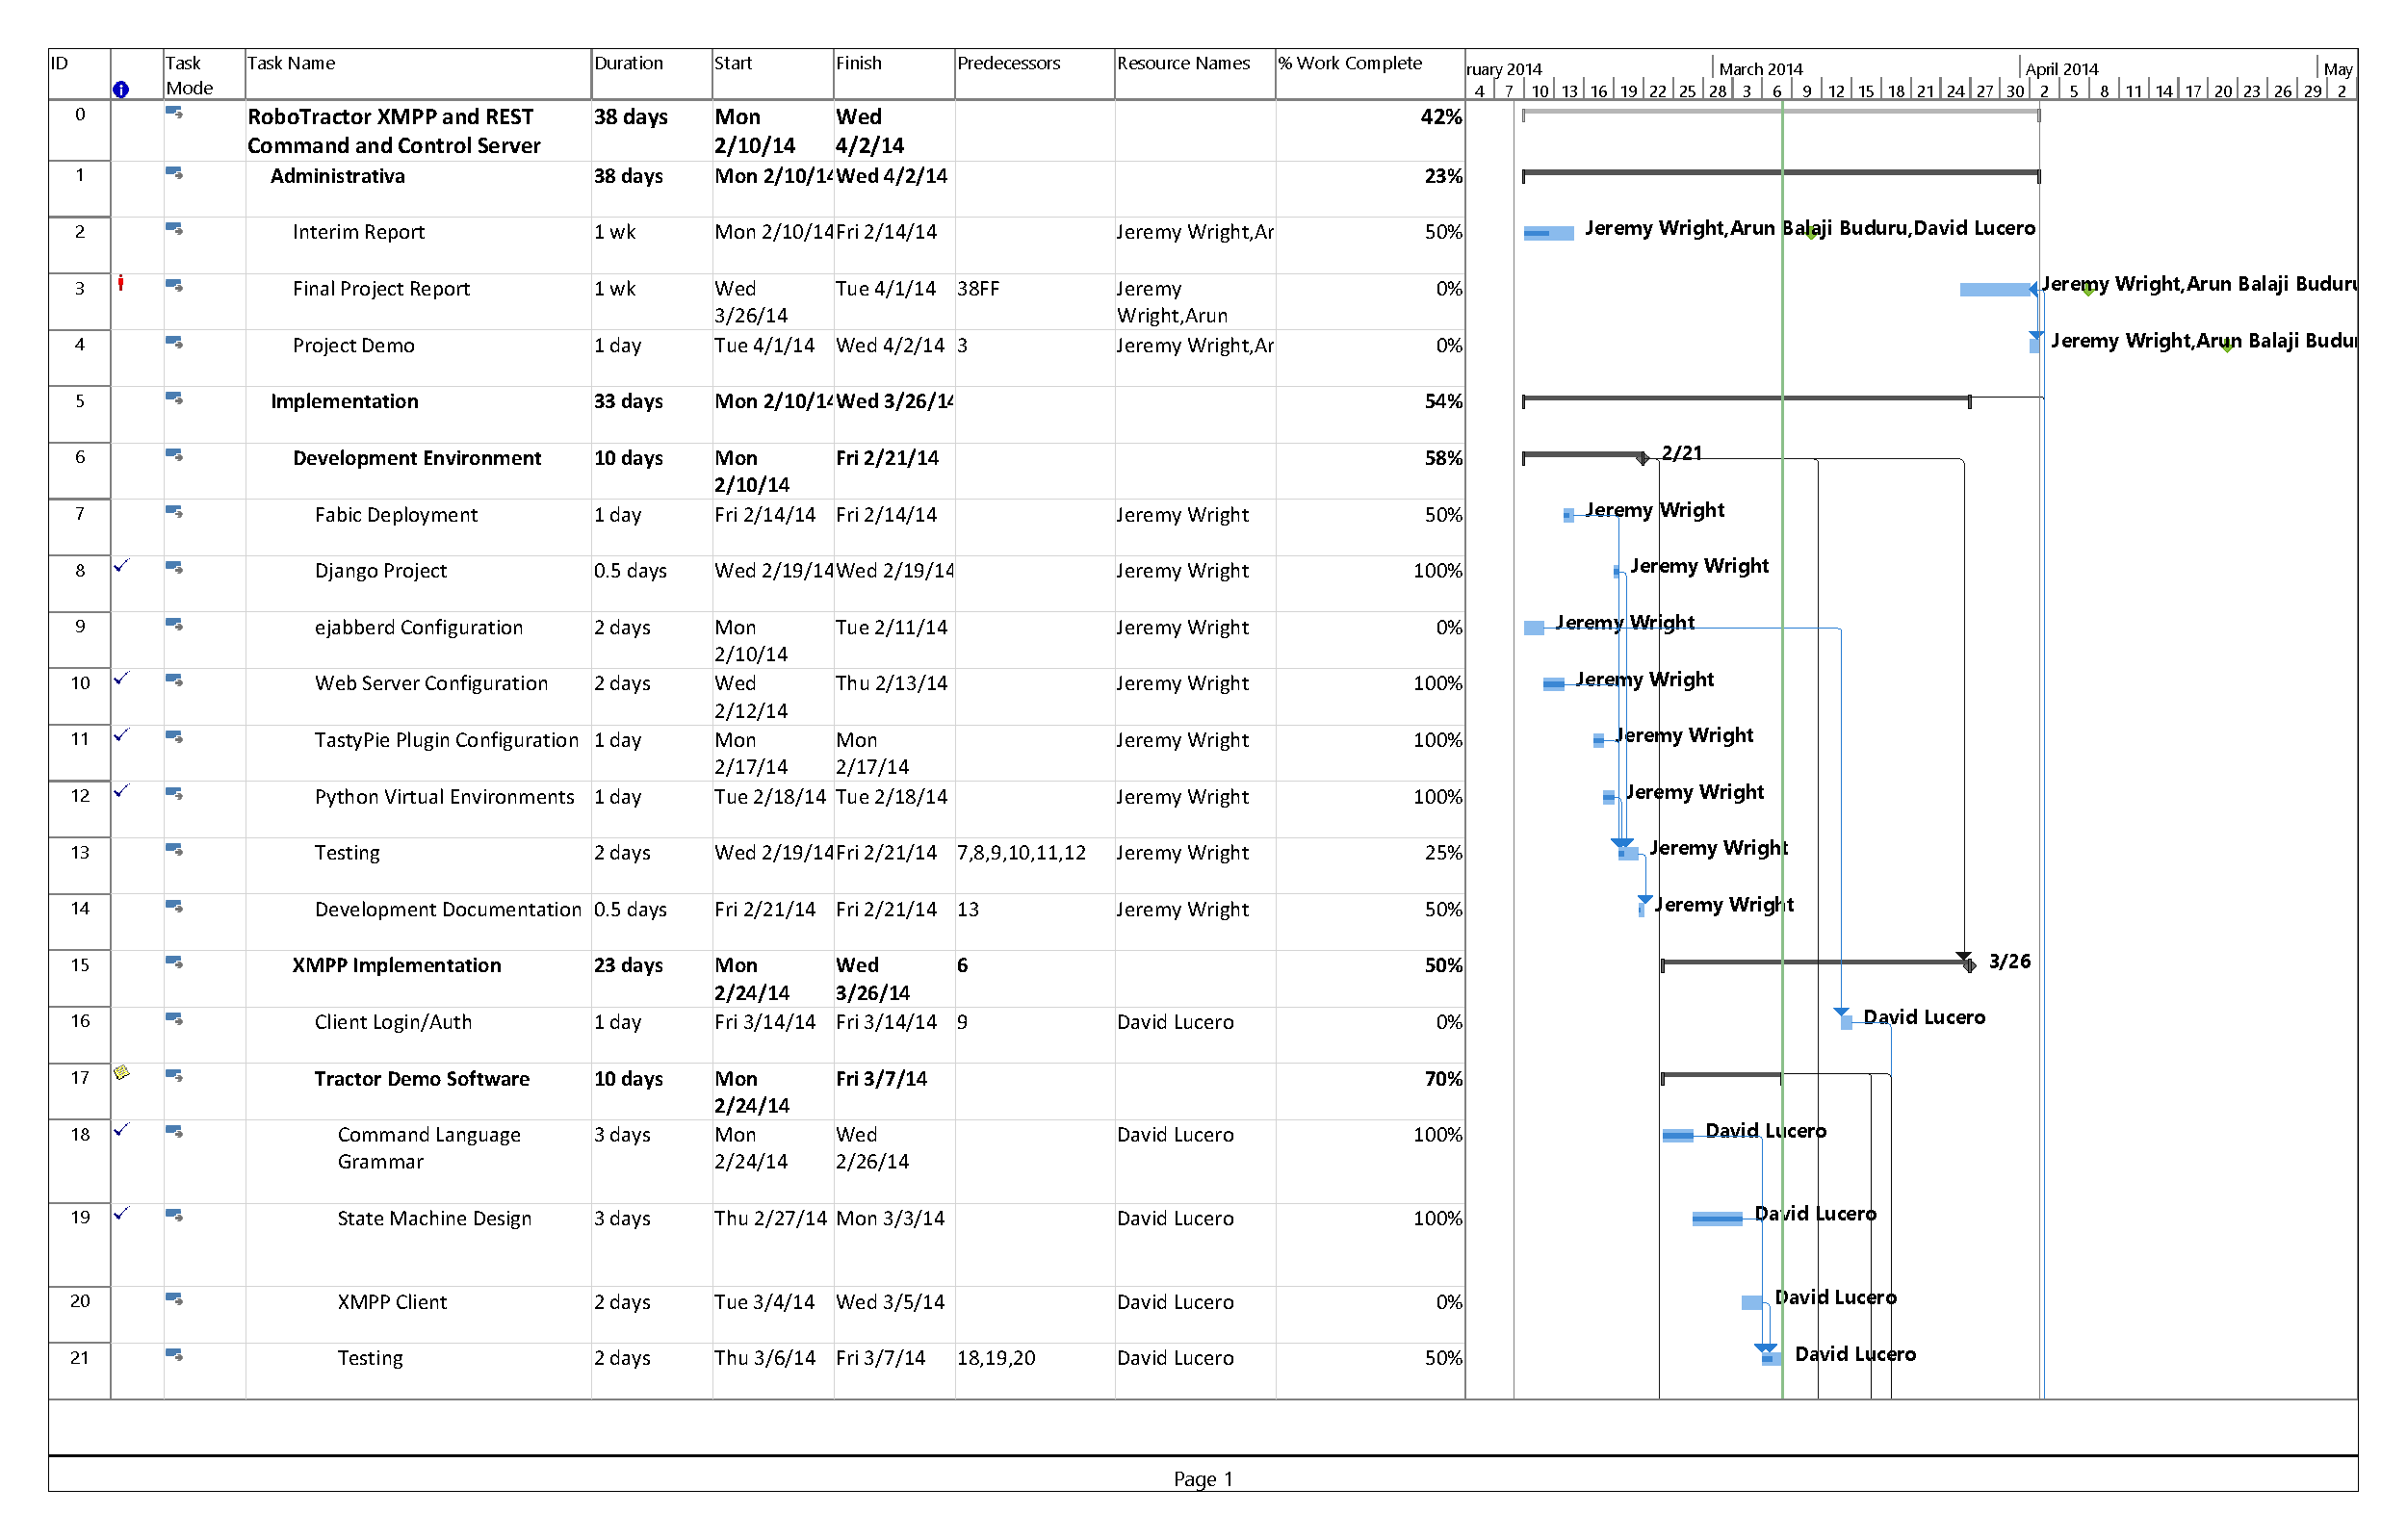
\includepdf[pages=-,landscape=true]{schedule.pdf}
 \DIFaddend\end{document}


